\chapter{Evaluación}
\label{cap:evaluacion}

En este capítulo se describe la evaluación de la aplicación que se ha llevado a cabo. Como ya se puso de manifiesto en el Plan de trabajo (ver Sección \ref{sec:planTrabajo}), la idea inicial era la de realizar una evaluación con usuarios finales y, preferiblemente, en la Facultad de Informática de la UCM, pues ese espacio es nuestro caso de estudio inicial. Debido a la crisis sanitaria y el estado de emergencia declarado en marzo de 2020 a causa del COVID-19, no ha sido posible la ejecución dicha evaluación. Sin embargo, se ha adaptado, en la medida de lo posible, el plan de evaluación. En las secciones que siguen se detalla cómo se ha llevado a cabo la adaptación tanto del plan de evaluación como la aplicación a otro edificio, destacando así su generalidad. 

LA INTRO CONTINUARÁ CUANDO ESTÉ EL CAPÍTULO ACABADO


\section{Adaptación de la aplicación a un nuevo edificio}

En esta sección detallaremos los cambios que se deben realizar para poder utilizar la aplicación Blind Bit en un edificio nuevo. El código tanto del servidor como del cliente se han implementado de tal manera que la información relativa al edificio sobre el que se despliega quede reducida a la información contenida en archivos xml que no forman parte del código. Sin embargo, son algunas las consideraciones que hay que tener en cuenta antes de comenzar con el mapeo de un nuevo espacio. 

\subsection{Cambios en el servidor}
\label{sub:cambiosServidor}

Como se puso de manifiesto en la Sección \ref{sec:servidor}, la información sobre la estructura del edificio que emplea el servidor para el cálculo de la ruta está contenida en los archivos xml y json correspondientes (ver Sección \ref{sec:mapeo}). Gracias a los archivos xml, el servidor conoce los cuadrantes que hay en una planta y, por tanto, sabe identificar cuándo hay que hacer un cambio de planta. Además conoce la dirección en la que se mueve el usuario ya que sabe la dirección de conexión de los cuadrantes. Así mismo, permite indicar al usuario hacia qué dirección se encuentra su destino en función del camino que haya seguido para llegar a él. De esta manera, el código que genera la ruta es totalmente independiente del edificio. Tan solo se espera que el cambio de planta se haga por medio de un ascensor, lo que parece de esperar cuando se mapean lugares como una facultad o un museo. Además, los ascensores suelen estar adaptados con escritura en braille. A continuación se detallan las claves para hacer el mapeo de un nuevo edificio.

\subsubsection{Mapeo de un nuevo edificio}

TE LA DEJO A TI QUE ERES MÁS EXPERTA



\subsection{Cambios en el cliente}

En las Secciones \ref{sub:diseño} y \ref{sub:func_cliente}, revisamos el diseño de la interfaz de la aplicación Blind Bit y su funcionamiento, respectivamente. En cuanto a la interfaz se refiere, es sencillo darse cuenta de que la parte dependiente del edificio corresponde a la pantalla de destinos. Sin embargo, esta está implementada de manera dinámica. Es decir, los nombres de los botones, así como la lista de destinos con la etiqueta correspondiente a los destinos tal y como aparecen en el archivo \textit{destinos.json} del servidor\footnote{Los destinos en la interfaz pueden aparecer con tildes, mayúsculas y otros caracteres especiales que puede no ser posible añadir en el archivo \textit{destinos.json}. Es por ello que se guardan los destinos en dos estructuras, una para la interfaz y otra para la conexión con el servidor.} se guardan en un archivo xml. El archivo donde se guardan estos y otros strings correspondientes a la aplicación, tales como el texto de las instrucciones o la uri del servidor es \textit{listasStringsApp.xml}. Las estructuras referentes a la lista de destinos son \textit{destinos\_array} y \textit{destinosdinamicos\_array}. Mientras que en la primera basta con introducir cada destino en un \textit{<item>}, en la segunda hay que indicar si ese destino tiene un segundo nivel. Por ejemplo, en el caso de la Facultad de Informática tenemos un botón aulas, que no corresponde con un destino sino con el acceso a un segundo nivel donde se muestran las aulas destino disponibles. La estructura que debe seguirse es la siguiente: 


\lstinputlisting[language=XML]{Imagenes/Evaluacion/destinos_array.xml} 

\lstinputlisting[language=XML]{Imagenes/Evaluacion/destinosdinamicos_array.xml}

Donde un ``no'' tras la barra indica que no hay un segundo nivel y cualquier otra cadena de strings se entiende como los destinos correspondientes a ese nivel, separados por comas.

\section{Objetivos de la evaluación}

Debido a la imposibilidad de realizar una evaluación con usuarios, como era el plan inicial, tras la declaración del estado de alarma en marzo de 2020 a causa del COVID-19 y el cierre de la Facultad de Informática de la UCM, nos vimos obligadas a reestructurar el \textit{modus operandi} de la evaluación de la aplicación. Concretamente, los objetivos cambiaron, centrándose en el funcionamiento de la misma y dando menos peso a la usabilidad, en la que los usuarios finales tienen un papel decisivo. De esta manera, se decidió establecer cuatro objetivos claros que presentamos a continuación:

\begin{enumerate}
	
	\item \textit{Resolución del problema del posicionamiento:} Una de las funcionalidades principales de la aplicación es, sin duda, la correcta ubicación del usuario. Para ello es necesario que el \textit{beacon} más cercano al usuario sea detectado como el más cercano por la aplicación (ver Sección \ref{sub:func_cliente}). De esta tarea depende no solo el inicio de la ruta sino el seguimiento de toda ella, pues en todo momento debemos conocer el cuadrante donde se encuentra el usuario para que la aplicación pueda responder en consecuencia. Una mala ubicación del usuario podría provocar que el usuario se pierda debido a indicaciones que no corresponden con la posición del usuario o, en casos más graves, el tropiezo o golpeo del usuario con un obstáculo del que no ha sido advertido.
	
	En el posicionamiento influye no solo la correcta implementación del código, sino también la ubicación de los \textit{beacons}, que debe adaptarse a las necesidades específicas de cada edificio. 
	
	\item \textit{Generación de instrucciones correctas:} Teniendo en cuenta la ubicación del usuario y el camino que ha seguido, es primordial que la aplicación sea capaz de generar instrucciones correctas. Tanto los giros como la señalización de puntos de interés como los ascensores o el destino debe corresponderse con la ubicación real de estos, tal y como se establece en los archivos xml (ver Sección \ref{sub:mapeo_xml}).
	
	\item \textit{Precisión de las instrucciones:} Además de que las instrucciones sean correctas, hay que evaluar que el usuario las recibe en el momento adecuado. Esto está claramente relacionado con el posicionamiento, pues el momento de indicación de la ruta se basa en cuándo el usuario llega a un determinado cuadrante. Sin embargo, se debe prestar especial atención a las posibles variaciones que pueden darse (una instrucción puede darse con cierta antelación o, por el contrario, una vez pasado el punto óptimo) y evaluar si esa flexibilidad es asumible para el usuario.
	
	\item \textit{Ejecución correcta en caso de usuario perdido:} Este es un punto importante, pues no debemos asumir que el usuario va a seguir siempre la ruta, puede ocurrir que por diversos motivos (una distracción, un obstáculo o el propio fallo de la aplicación) el usuario se desvíe de la ruta. En ese caso no solo se debe identificar el problema sino también saber reconducir al usuario al destino deseado. 
		
\end{enumerate}


\section{Realización y resultados de la evaluación}

La realización de la evaluación no pudo darse en el edificio objetivo de nuestro estudio (la Facultad de Informática de la UCM) debido a la imposibilidad de acceder a él. Sin embargo, conseguimos sobreponernos a este contratiempo y poner de manifiesto la flexibilidad de la aplicación mapeando otro edificio y realizando diversas pruebas sobre este. Este edificio no pudo ser otro que una vivienda. Cabe destacar que este no es el escenario ideal sobre el que se desplegaría una aplicación como Blind Bit, pues el espacio queda considerablemente reducido en comparación con el de una facultad o museo, por ejemplo. A pesar de ello, permite probar el comportamiento de la aplicación en situaciones donde cierta aglomeración de \textit{beacons} es necesaria y poner a prueba el mapeo de un edifico con características distintas al ya planteado en la Sección \ref{sec:mapeo}.

\subsection{Mapeo del nuevo espacio}

Como ya se avanzaba en la introducción, el edificio sobre el que se basa la evaluación es una vivienda. En la Figura \ref{fig:mapeoCasa} vemos el resultado del mapeo, donde el número de cuadrante está en el recuadro negro, la posición de los beacons en amarillo y los cuadrantes vienen delimitados por las líneas rojas y las paredes de la vivienda. Como muestra la Figura \ref{fig:mapeoCasaPAlta}, el mapeo de la planta alta se ha reducido a dos cuadrantes, pues son suficientes para \textit{testear} las rutas que incluyen un cambio de planta ya que la estructura es análoga a la de la planta baja.


\begin{figure}[h!]
	\centering
	
	\subfloat[Mapeo de la planta baja de la vivienda]{
		\label{fig:mapeoCasaPBaja}
		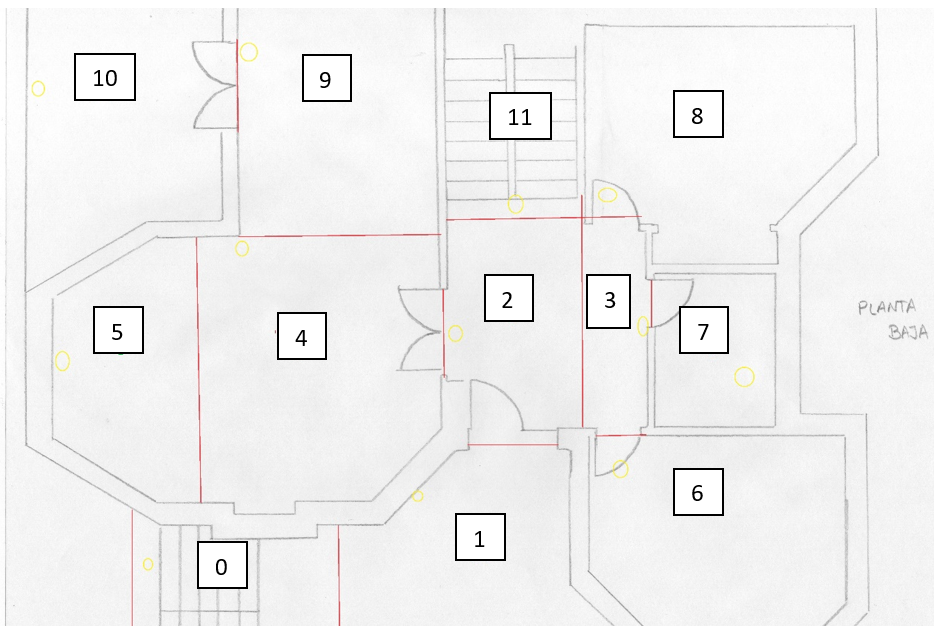
\includegraphics[width=0.8\textwidth]{Imagenes/Evaluacion/planoCasaPBaja}}
	
	\subfloat[Mapeo de la planta alta de la vivienda]{
		\label{fig:mapeoCasaPAlta}
		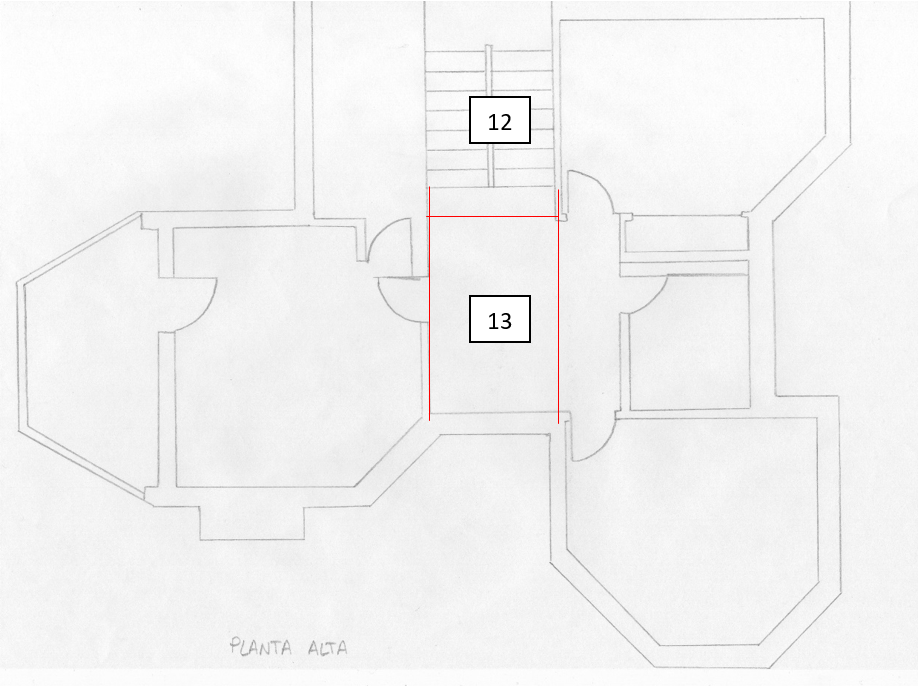
\includegraphics[width=0.8\textwidth]{Imagenes/Evaluacion/planoCasaPAlta}}\\
	
	\caption{Mapeo de la vivienda}
	\label{fig:mapeoCasa}
\end{figure}

%	
%\begin{figure}[t]
%	\centering
%	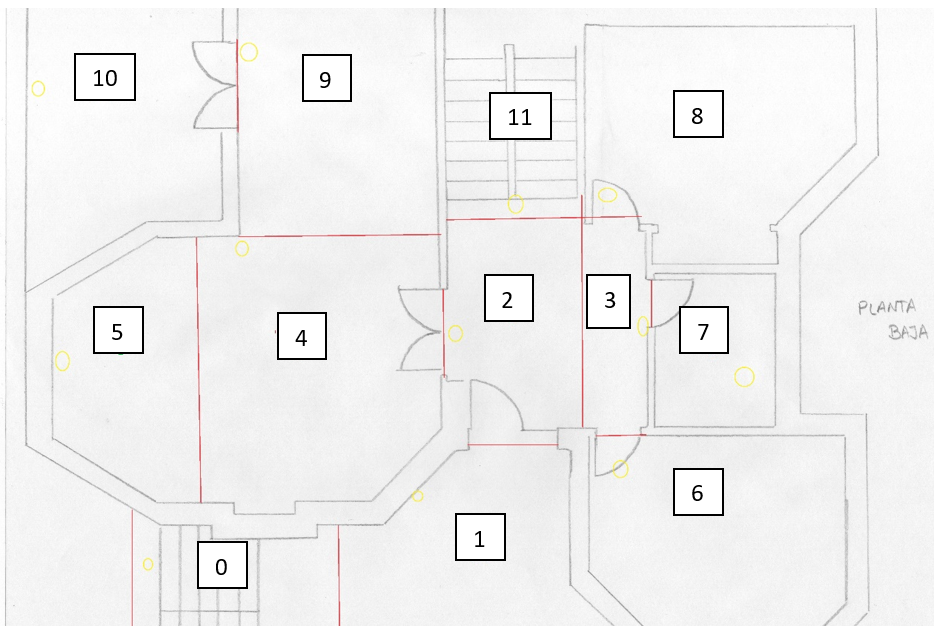
\includegraphics[width=0.9\textwidth]{Imagenes/Evaluacion/planoCasaPBaja}
%	\caption{Mapeo de la planta baja de la vivienda.}
%	\label{fig:mapeoCasaPBaja}
%\end{figure}
%
%
%\begin{figure}[t]
%	\centering
%	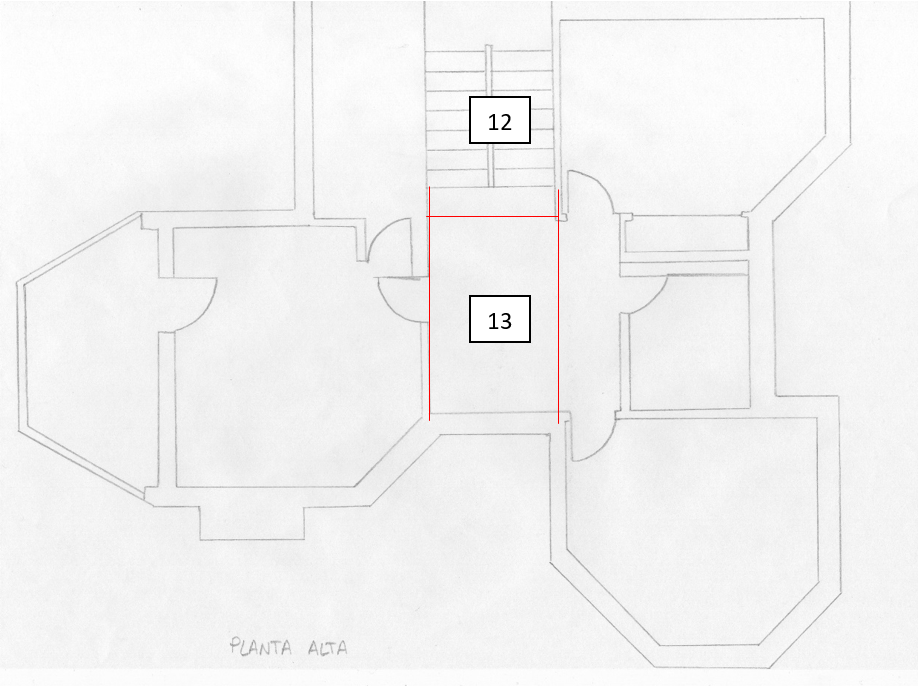
\includegraphics[width=0.9\textwidth]{Imagenes/Evaluacion/planoCasaPAlta}
%	\caption{Mapeo de la planta alta de la vivienda.}
%	\label{fig:mapeoCasaPAlta}
%\end{figure}



A continuación se describen las pruebas realizadas y se analizan los resultados obtenidos.

\subsection{Seguimiento de la ruta}
En esta sección se detallan las pruebas realizadas asumiendo que el usuario no va a salir de la ruta. Sin embargo, algunas de ellas están diseñadas para reproducir situaciones extremas como la pérdida de un \textit{beacon} o rutas potencialmente complicadas.


\subsubsection{Ruta del cuadrante $0$ al cuadrante $10$}
\label{subsub:0al10}
La primera ruta de la evaluación consiste en realizar la ruta desde el cuadrante $0$ hasta el cuadrante $10$ sin salir de la ruta. En esta se debe prestar especialmente atención a las instrucciones de giro, pues son constantes durante toda la ruta. Además, no debemos olvidar que la aplicación emite distintas vibraciones en función de la dirección de giro. Estas vibraciones deben quedar lo suficientemente claras para el usuario. 

Este recorrido se realizó varias veces a fin de encontrar irregularidades en la ruta. A continuación se detallan las conclusiones obtenidas:

\begin{itemize}
	\item Las instrucciones generadas por la aplicación son correctas y, en la mayor parte de los casos, se indican al usuario en el momento adecuado.
	
	\item Las vibraciones asociadas a los giros y a la llegada del destino son lo suficientemente distintas para que el usuario pueda distinguirlas.
	
	\item En dos ocasiones las instrucciones correspondientes a los cuadrantes $1$ y $2$ se dieron demasiado pronto. Esto puede deberse a que el \textit{beacon} del cuadrante $1$ está situado en el exterior y que, una vez que se avanza hacia la puerta que separa los cuadrantes $1$ y $2$, la distancia que hay entre ellos es reducida.
	
	\item En una de las ocasiones el \textit{beacon} asociado al cuadrante $4$ no fue detectado por la aplicación, provocando la pérdida de esa instrucción (en las pruebas siguientes se detalla el comportamiento de la aplicación en este caso. Ver Secciones \ref{subsub:0al10sin4} y \ref{sub:usuarioPerdido}).
	
	\item Una vez se ha llegado al destino, la posición del mismo se indica correctamente en función de la dirección desde la que venga del usuario.
	
\end{itemize}

\subsubsection{Ruta del cuadrante $1$ al cuadrante $10$}

Este caso es prácticamente idéntico al anterior (Sección \ref{subsub:0al10}), con la única diferencia que se pone a prueba el posicionamiento inicial del usuario. Tras comprobar que las instrucciones en el cuadrante $1$ se daban antes de lo previsto en algunas ocasiones, se decidió empezar la ruta en este cuadrante. De esta manera la aplicación debía detectar el \textit{beacon$1$} como \textit{beacon} más cercano. Se hicieron cinco pruebas y se pudo comprobar que en dos ocasiones este posicionamiento no se realizó de manera correcta. En uno de ellos el \textit{beacon} más cercano detectado por la aplicación fue el $4$ (lo que puede ser provocado porque la separación entre el $4$ y el $1$ es una ventana) y en otro el $2$ (cuya posible explicación está en la sección anterior).

\subsubsection{Ruta del cuadrante $0$ al cuadrante $10$, eliminando el \textit{beacon} del cuadrante $4$}
\label{subsub:0al10sin4}

En este caso se ha vuelto a repetir la ruta del cuadrante $0$ al $10$ con la particularidad de que el \textit{beacon$4$}\footnote{Asumiremos que \textit{beaconX} es el \textit{beacon} asociado al cuadrante X.} fue eliminado de la ruta. Sin embargo, no provocamos la situación de que el usuario se saliera de la ruta (como sería lógico en esta situación, pues la instrucción de giro del cuadrante $4$ se pierde), continuamos por el cuadrante $9$. De esta manera la aplicación no notifica que el usuario se ha perdido, pues sigue en la ruta. A pesar de que la instrucción indicada en el cuadrante $9$ fue la correcta (giro a la izquierda), la aplicación tardó demasiado. Esto se debe a que la variable \textit{numPasosPerdidos}, que identifica el momento en el que el usuario puede haberse perdido (ver Sección \ref{sub:func_cliente}), es demasiado elevada para este edificio, donde las distancias entre \textit{beacons} son pequeñas.


\subsubsection{Ruta del cuadrante $1$ al cuadrante $5$, eliminando el \textit{beacon} del cuadrante $2$}

Este caso es interesante, pues, a pesar de que se ha eliminado uno de los \textit{beacons} correspondientes a una intersección, la información de giro en el cuadrante $2$ no se pierde. Esto se debe a que, como la aplicación es capaz de avisar de los cambios de dirección con antelación, en el cuadrante $1$ ya se indica al usuario que, tras avanzar unos metros, debe girar a la izquierda. Bien es cierto que se pierde precisión, pues el usuario no percibe la instrucción de giro en el momento en el que debe realizarse, ni la confirmación sonora y vibración asociada a esta. Sin embargo, el hecho de que se den instrucciones por adelantado favorece que el usuario permanezca en la ruta aún cuando alguna instrucción se pierda. 

Particularmente para esta ruta, el giro del cuadrante $2$ es el único que hay que realizar y, debido a esto, es más fácil que el usuario no se pierda. Si, por el contrario, el destino hubiera sido el cuadrante $10$, es probable que el usuario no hubiera llegado a recibir la instrucción de giro a la derecha del cuadrante $4$ tampoco. Esto se debe a que la aplicación necesita un tiempo (llegar a un número de pasos perdidos) para decidir si el usuario se ha perdido. De esta manera, cuando el usuario llega al cuadrante $4$ la aplicación sigue a la espera del cuadrante $2$. Esto implica que el usuario se salga de la ruta. Caso que abordamos en la siguiente sección.


\subsubsection{Ruta del cuadrante $1$ al cuadrante $13$}

En este caso, lo que se quería evaluar era las instrucciones del cambio de planta. Como ya se comentó en la Sección \ref{sub:cambiosServidor}, el código asume que los cambios de planta se realizan por medio de ascensores. Esta información se ha ignorado en esta ocasión, pues solo se disponía de escaleras. 

De la ruta desde el cuadrante $1$ al $13$ destacamos un punto importante, que es la anticipación de los ascensores en el cuadrante $2$ gracias a la información adicional generada. Esto avisa al usuario del cambio de planta. Una vez en el cuadrante $13$, la aplicación indica al usuario a qué planta se debe dirigir y en qué dirección se encuentran los ascensores (en este caso, delante del usuario). Una vez en la planta superior, la instrucción del cuadrante 12 continua teniendo en cuenta la nueva orientación del usuario (continúa recto). 

\subsubsection{Ruta del cuadrante $13$ al cuadrante $8$}

La finalidad de esta ruta es, principalmente, comprobar el comportamiento de la aplicación en el \textit{hall} de la planta baja, así como el cambio de planta inverso. 

El problema que surge aquí es que los giros que hay que realizar en la planta baja son bastante tediosos. Por un lado, la ubicación del \textit{beacon$2$} favorece que la instrucción de giro hacia el \textit{beacon$3$} tarde demasiado en llegar. Una vez que se proporciona esta instrucción, el cuadrante $3$ vuelve a hacer girar al usuario hacia el $8$, lo que provoca cierta confusión. De igual manera se probó la ruta inversa, desde el cuadrante $8$ al $13$, y el resultado fue análogo.


\subsubsection{Ruta del cuadrante $9$ al cuadrante $13$}

Como la ruta por el \textit{hall} de la planta baja había resultado tediosa en el caso anterior, se hizo una prueba desde el otro extremo. Esta vez la ubicación del \textit{beacon$2$} favorece el giro del usuario para encontrar el ascensor (escaleras en este caso). De esta manera la ruta resulta mucho más natural y organizada que en el caso anterior.

\subsection{Usuario perdido}
\label{sub:usuarioPerdido}

En esta sección se expone el comportamiento de la aplicación cuando el usuario sale de la ruta, basado en ejemplos de ejecución reales. 

En la Sección \ref{subsub:0al10sin4} vimos un caso en el cual era probable que un usuario se desviara de la ruta, debido a la pérdida de la instrucción de giro asociada al cuadrante $4$. De esta manera el usuario continuaría hasta llegar al cuadrante $5$. Es entonces cuando la aplicación detecta que el usuario se ha salido de la ruta e indica al usuario que debe volver por la dirección en la que venía y le permite iniciar de nuevo la ruta al destino desde su posición actual. Como ya se ha comentado, esta indicación se da con cierto retraso debido a que el valor que debe alcanzar la variable \textit{numPasosPerdidos} es demasiado elevada para este edificio. 


\section{Conclusiones}


